\section{Atomfysik} 



\footnote{Videor relevanta till kapitel \ref{sec:atomfysik}: \href{https://www.youtube.com/playlist?list=PL2ub1_oKCn7ogaMtdB2RumlIYqNeXf_oX}{Khan Academy, Semiconductors, videor 1-4.}}
\label{sec:atomfysik}
Pauli's Exclusion Principle states that no two electrons in the same atom can have identical values for all four of their quantum numbers. In other words, (1) no more than two electrons can occupy the same orbital and (2) two electrons in the same orbital must have opposite spins

\begin{figure}[ht]
    \centering
    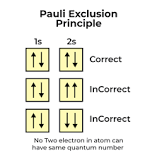
\includegraphics{bilder/fig:pauli.png}
    \caption{Pauli's exclusion principle}
    \label{fig:paulis}
\end{figure}

\begin{itemize}
    \item Bra ledare $\implies$ Många fria elektroner.
    \item Halvledare $\implies$ Väldigt få fria elektroner.
    \item Isolatorer $\implies$ I princip 0 fria elektroner.
\end{itemize} 

\subsection{Energinivåer}
Enligt Pauli kan inga två atomer ha samma energinivå. Dock kan en atom ha positiv eller negativ 'spinn' och då kan 2 elektroner få plats på samma energinivå, visat nedan i figur \ref{fig:Energinivåer}.

\begin{figure}[ht]
    \centering
    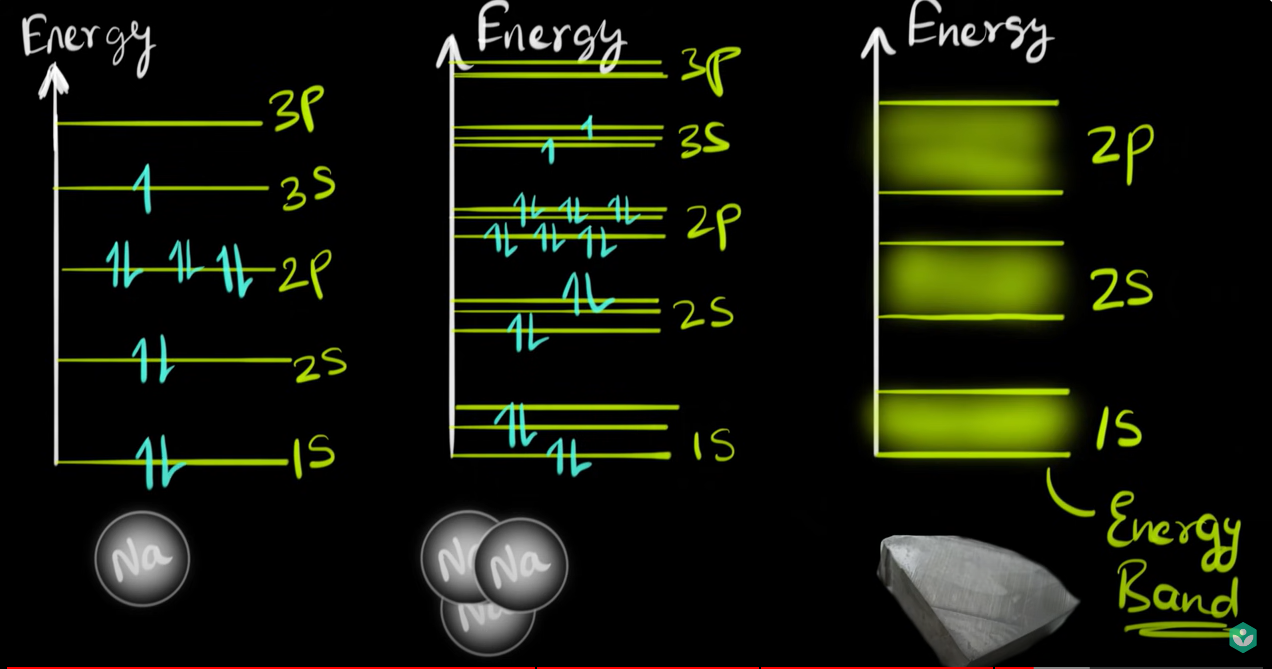
\includegraphics[scale = 0.3]{bilder/fig:energi.png}
    \caption{Energinivåer}
    \label{fig:Energinivåer}
\end{figure}

Ovan ser man visuellt hur en Natriumatoms energikonfiguration ser ut. De blåa pilarna är en atom vardera, med spinn åt olika håll. Olika nivåer (1S, 2S, 2P...) får plats med olika många atomer. Andra grafen visar hur en natriummolekyls elektronkonfiguration ser ut. Som man ser i andra grafen skapas flera orbitalnivåer på varje steg (1S, 2S, 2P...). Dessa brukar kallas 1S*, 2S* osv. Kombinationen av streck på varje orbitalnivå i andra grafen föreställer de nyskapade orbitalnivåerna för en molekyl. I fasta material har vi en enormt hög koncentration av atomer, vilket således leder till enormt många orbitalnivåer på varje steg 1S, 2S... Detta illustreras i grafen till höger. Vad som i den grafen är ritat som ett 'moln' är egentligen enormt många individuella orbitalnivåer, allt enligt Paulis princip (\ref{sec: pauli}). Detta 'moln' kallas för 'energiband'. Eftersom att varje energinivå kan hålla 2 elektroner (positiv och negativ spinn), kan varje energiband med \textit{N} antal energinivåer bära \textit{2N} antal elektroner.

Varje orbital 1S, 2S... kan hålla olika antal elektroner. 
\begin{itemize}
    \item s-orbital: Varje s-orbital kan hålla upp till 2 elektroner.
    \item p-orbital: Varje p-undernivå kan hålla upp till 6 elektroner (3 olika orbitaler, var och en med plats för 2 elektroner).
    \item d-orbital: Varje d-undernivå kan hålla upp till 10 elektroner (5 olika orbitaler, var och en med plats för 2 elektroner).
    \item f-orbital: Varje f-undernivå kan hålla upp till 14 elektroner (7 olika orbitaler, var och en med plats för 2 elektroner).
\end{itemize}

\begin{figure}[ht]
    \centering
    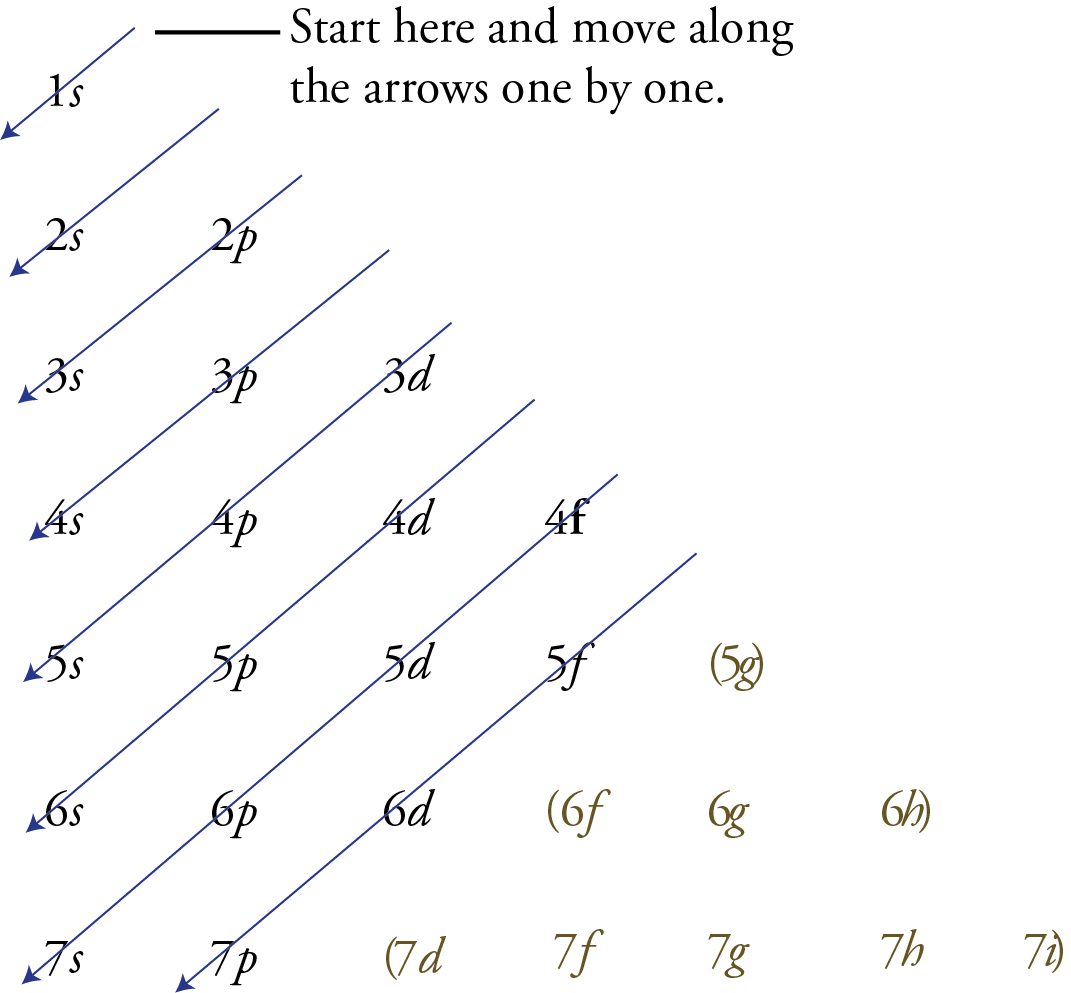
\includegraphics{bilder/fig:elektronkonfig.png}
    \caption{Orbitalnivåer och dess förmåga att hålla elektroner.}
    \label{fig:orbitalnivåer}
\end{figure}

Varje streck i figur \ref{fig:Energinivåer} visar ett atomskal i ordning K,L,M,N där om man summerar antalet elektroner varje orbitalnivå kan hålla kommer fram till att de respektive skalen kan hålla 2, 8, 18, 32 elektroner. Exempelvis kan alltså 'strecket' som går över 3d, 4p, 5s bära $10 + 6 + 2 = 18$ elektroner. Det strecket representerar således ett M-skal.



Det krävs energi för en elektron att kunna röra sig mellan orbitalnivåer. En temperaturökning kan vara någonting som tillför denna energin. I material som vi kallar för ledare, överlappar orbitalnivåerna varandra, och gapet, $E_g$, försvinner. Istället får vi ett enda stort band där elektroner kan röra sig fritt, vilket illustreras i den vänstra grafen i figur \ref{fig: valens_ledningsband}. För isolatorer är detta bandgap väldigt stort villket försvårar elektronrörelse, och för halvledare är det lite mittemellansvårt. Ledare, isolatorer, och halvledare definieras utifrån storleken på detta gap enligt följande:

\begin{equation}
    \begin{cases}
       & {Ledare: E_g < 0 eV} \\
       & {Halvledare: 0 eV < E_g < 2 eV} \\
       & {Isolatorer: E_g > 4 eV}
    \end{cases}       
\end{equation}

Dessa definitionerna lämnar lite utrymme vad gäller energinivåer som krävs för elektronövergång men jag gissar att man inte vill använda de materialen bara för att de är både kassa halvledare \textit{och} kassa isolatorer.

Valensband är definierat som det högsta fyllda bandet vid 0 K (måste inte vara helt fyllt). Det näst högsta bandet heter ledningsbandet. För en ledare har man bara ett stort band, därför kallar man det oftast inte för något av valens/ledningsband. 

\begin{figure}[ht]
    \centering
    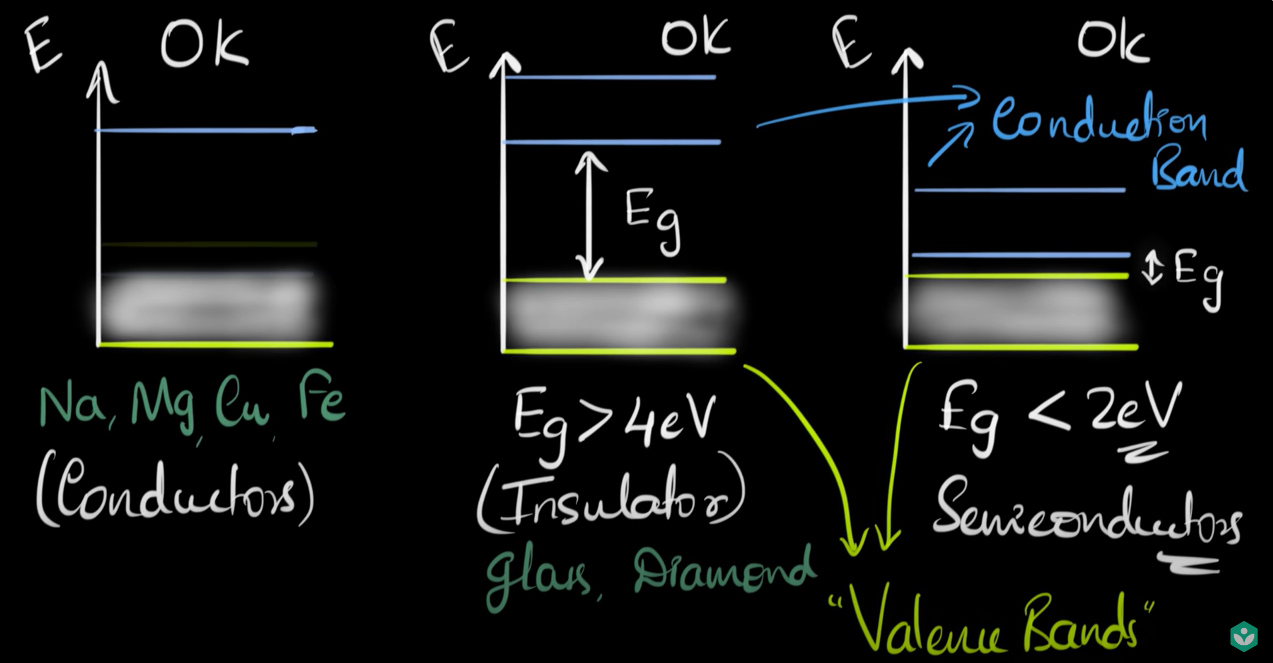
\includegraphics[scale = 0.3]{bilder/gap_iso_halvledare_ledare.PNG}
    \caption{Valensband och ledningsband för ledare, isolatorer, och halvledare.}
    \label{fig: valens_ledningsband}
\end{figure}

